\chapter{Discussion}

This section will assess the performance of strain estimation algorithms by examining key unwrapping techniques and strain estimators in the context of the three metrics for this work: processing time, sensitivity and image resolution, as well as the overall quality and characteristics of the image. 
The results discussed are based on the contributions of the two major processes in strain estimation: the phase unwrapper, and the strain estimator. However, it should be noted that the resulting performance of each strain estimation algorithm is a result of its particular combination of these two factors, for which the contributions can only be marginally separated.

This discussion will point towards an optimum strain estimation algorithm, in the context of the data set imaged and the motivation for this work. 

\section{Phase Unwrapping}

Examining the B-scan images in \autoref{bscan_images_1} and \autoref{images} show that the techniques that utilise the volume phase unwrapping algorithm all exhibit artefacts in the region of low signal directly below the inclusion. This is echoed in the \ac{fd} methods to an extent, but are quite clearly not visible in the \ac{posg}. Examining images at lower strain filter \ac{fwhm} show that the phase offset still produces noise in these regions. 

Beyond these concerns, even when applying the \ac{sg} filter as a convolution to the unwrapped phase, the strain estimation processing does not allow more than a 10$\times$ speed up over the \ac{uwwls} technique (for 3D processing), and with little improvement in image quality. Alongside this, the need to read in the data set in order to unwrap it over multiple B-scans is a significant limitations to further applications of parallel processing.

Applying a phase offset, as per \cite{zaitsev_hybrid_2016}, does appear to be faster than the unwrapping algorithm when processing the 3D data set, and also decreases the noise artefacts seen below the inclusion in the low \ac{snr} region. It performs on the same order in sensitivity as the \ac{uwsg}, which is still worse than the \ac{uwwls} and the unweighted \ac{fd} techniques. Although a useful proof of concept, it does not appear to add significant improvements in either processing speed or sensitivity in comparison to the \ac{fd} techniques that remove the need for phase unwrapping altogether. In addition, the phase offset performed poorly in regards to image resolution. Looking at the \ac{uwsg} algorithm in comparison, which used the same strain estimator but a different phase unwrapping technique, the loss of image resolution must be traced back to the phase offset unwrapping method applied.

\section{Strain Estimator}

The \ac{sg} filter strain estimators performed as expected: at slightly less sensitivity than the \ac{wls} estimator, although their ability to be applied as a convolution did result in a ~10$\times$ speed up. Surprisingly, use of \ac{ols} in \ac{uwsg} significantly improved the axial resolution with the unwrapping algorithm compared to the \ac{wls}. Both \ac{posg} and \ac{uwsg} techniques that utilised the filter showed streak patterns across certain strain filter \ac{fwhm} values in the lateral image resolution, suggesting that optimal filter sizes exist (at least for this phantom data). 

What was particularly surprising was how poorly the \ac{wfd} technique performed in the image quality metrics. This technique presented strong artefacts in comparison to other images, and had a degraded sensitivity and lateral image resolution, despite having significantly better axial resolutions, particularly at high strain filter \ac{fwhm} values than other techniques.
These results are surprising considering the fact the weighted smoothing was meant to compensate for noisy, and therefore inaccurate, data points, and instead showed significant artefacts. One reason as to why this hasn't appeared to work could be that our assumptions about the associated variances of the phase value are incorrect for this phantom. This could be if the scatterers were not evenly distributed within the bulk as they would be in tissue. The poor results for lateral resolution could be a result of one of these optical artefacts appearing in the region where the error function was fitted, and therefore exaggerating the image resolution.

Another way of approaching the problem with the \ac{wfd} strain estimator could be that instead of seeing these features as artefacts, since they were also observed in the \ac{oct} image and therefore exist physically in the phantom, that the technique increases contrast by weighting the optical component more heavily. The question to ask then, is if this is beneficial to the overall image. In the case of this phantom, and using metrics of sensitivity and image resolution, it appeared not. 

In response to these concerns, the \ac{pffd} strain estimator was implemented to try and smooth the influence of these high intensity optical features. As a result, the \ac{pffd} technique did show an increase in sensitivity above the \ac{wfd} (as well as all other techniques), and a better lateral image resolution. Because the strain and lateral smoothing filter were corrected for added smoothing performed by the pre-filter, the improvement in sensitivity must be a result of the combination of weighted and unweighted smoothing. It is interesting, but perhaps not surprising, to note that this technique also appeared to produce a combination of the patterns that appeared in both the \ac{wfd} and \ac{uwfd} image resolution plots. Although not significantly compared to the processing time of the \ac{uwwls}, the \ac{pffd} did show a slight increase in processing time compared to the other \ac{fd} methods, due to the double filter convolution that had to be applied.

The \ac{uwfd} algorithm performed well in all image quality metrics, and was among the other \ac{fd} techniques in having a significant improvement in processing speed. The resulting images look very similar to the \ac{wls} result, which is interesting considering this method did not make use of the optical weighting. 

What the results have shown is that the performance of the \ac{fd} strain estimator in terms of image quality metrics is highly dependent on the smoothing filter used in combination. However there is no doubt that these algorithms show the best improvement in processing speed. 

\section{Optimal Processing Algorithm}

Taking these results in conjunction with those regarding the unwrapping techniques in the sections above, it is decided that the \ac{uwfd} strain estimation algorithm provides optimal processing speed, sensitivity, and image resolution. In particular, using a strain filter \ac{fwhm} of 40$\mu$m and a lateral smoothing filter \ac{fwhm} of 20$\mu$m should provide the best axial and image resolution, in conjunction with high sensitivity. 

\begin{figure}
	\centering
	\begin{subfigure}{0.49\textwidth}
		\centering
		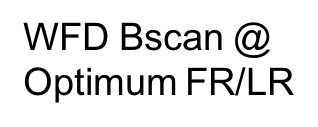
\includegraphics[width=\textwidth]{figures/uwfd_compare.png}
	\end{subfigure}
	\begin{subfigure}{0.49\textwidth}
		\centering
		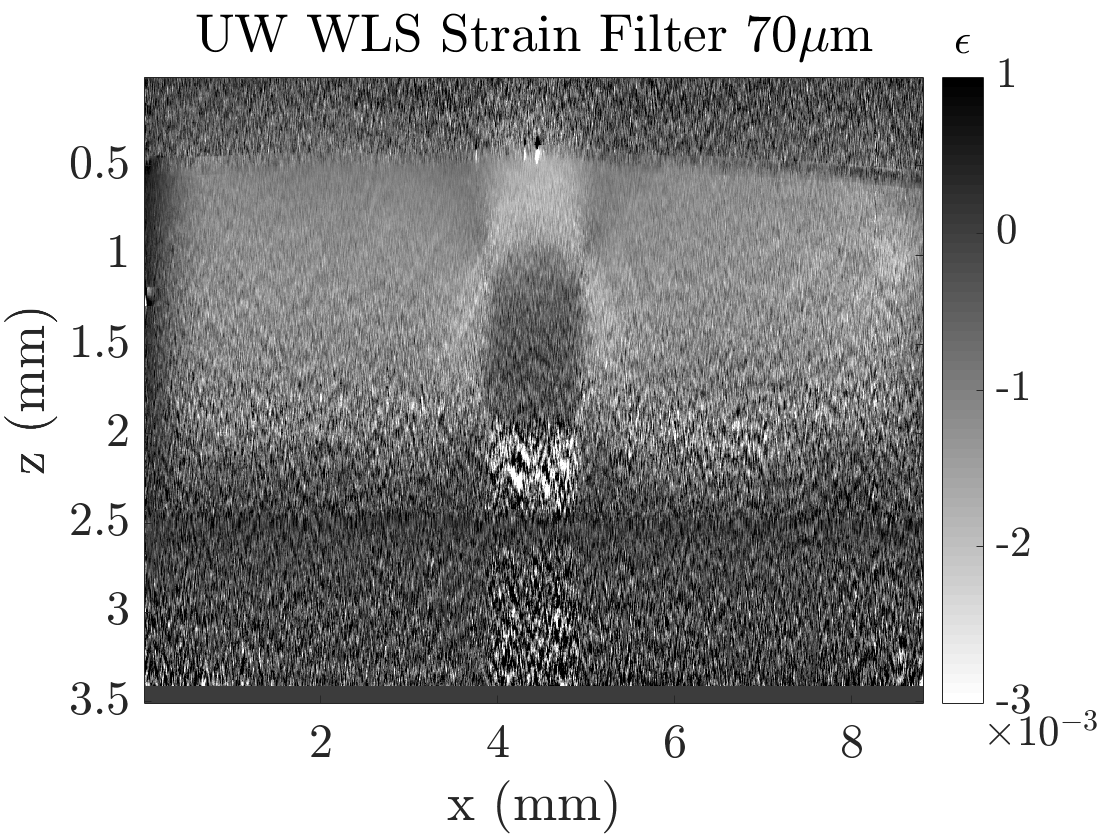
\includegraphics[width=\textwidth]{figures/wls_compare.png}
	\end{subfigure}
	\caption{\ac{uwfd} strain estimation B-scan compared with the previously standard unwrapping with \ac{uwwls}.}
	\label{wls_uwfd_compare}
\end{figure}

\autoref{comparison_table} shows that all image quality parameters are improved in comparison with the previously used \ac{uwwls} approach, at least for this particular phantom. It is important to note that the other strain estimation techniques performed very similarly in areas of sensitivity and relatively so in image resolution, therefore application on a different, less homogeneous phantom, or on an actual tissue sample, may prove another to be optimal.

\begin{table}
	\begin{tabularx}{\textwidth}{Yrrc}
		\toprule
		& \textbf{\ac{uwwls}} & \textbf{\ac{uwfd}} & \textbf{Improved?}\\
		\midrule 
		Strain Filter FWHM ($\mu$m) & 70 & 40 \\
		Lateral Smoothing Filter FWHM ($\mu$m) & 0 & 20 \\
		\midrule
		2D Processing Time (s) & & \\
		3D Processing Time (s) & 153.67 & \\
		Strain Sensitivity (m$\epsilon$) & 0.1607 & 0.1385 & 16\% \\
		Axial Image Resolution FWHM ($\mu$m) & 315.87 & 258.37 & \textbf{20\%} \\
		Lateral Image Resolution FWHM ($\mu$m) & 131.33 & 115.98 & 13\% \\
		\bottomrule
	\end{tabularx}
	\caption{Comparison of the previously standard \ac{uwwls} strain estimation technique and the optimised \ac{uwfd}.}
	\label{comparison_table}
\end{table}

The one result that has assured consistency across different data sets is the processing speed, which formed the main motivation for this work. All \ac{fd} based algorithms showed approximately a 50-100$\times$ speed up in strain estimation processing, which on the computer architecture used in the \ac{britelab} research group enabled a volume of 2.6$\text{mm}^2$ to be imaged in under 20 seconds.

\section{Future Work}

These results suggest many avenues for future work in phase-sensitive compression \ac{oce}. The process of fitting an error function to the boundaries in order to quantify the image resolution provided useful insights into the affects of averaging on different strain estimators, however the ease with which these results were obtained recommends interest in further possible application. For strain estimators that had high R-square values (such as those with lateral smoothing), and such had a robust error function fit, it may be possible to utilise an error function fitting process to routinely examine object boundaries. Examining the gradient between two objects might give insight onto what those objects actually are, particularly in the more heterogenous tissue samples. 

All strain estimators showed significant processing speed up against the \ac{uwwls}, however there is no reason to think their processing time limit has been reached. It has been discovered that \ac{gpu}s can greatly accelerate the processing of strain imaging for techniques such as ultrasound elastography that utilise speckle-tracking (rather than phase-sensitive measurement) \cite{peng_gpu-accelerated_2017}, therefore there is reason to believe this could also benefit in the phase-sensitive \ac{oce} case. Of particular benefit is the fact that all four strain estimation techniques that do not involve the volume phase unwrapping algorithm, are capable of processing individual B-scans completely independently, making it very likely that introducing parallel processing to these methods would significantly decrease the computation time. Applying filter convolutions (as in \ac{sg} filtering, and Gaussian smoothing in the \ac{fd} case) in parallel and on \ac{gpu}s could further improve the processing speed, towards intra-operative time frames, and even video-rate imaging. Before these possibilities are investigated however, the algorithms will likely need to be moved out of the Matlab interface, and applied in another language more suited to fast numerical processing.

The obvious next step for future work is to aim at translating this strain estimation algorithm into the clinic, by analysing its performance on a range of breast tissue samples. In particular, before being able to apply this technique to assess cancer margins during breast conserving surgery, diagnostic specificity and sensitivity (the ability to accurately differentiate healthy tissue from tumour) of the technique must be analysed using large case studies.

In conjunction with this, research also could be done in applying these strain estimation techniques to quantitative elastography imaging (imaging stress as well as strain), to determine which one is optimal. Measurement of a stress using a stress layer is relatively fast, and most of the computational burden falls on the strain estimation, therefore strain estimators that optimise the processing speed would benefit in this area also. 

